\pagenumbering{arabic} %設定頁號阿拉伯數字
\setcounter{page}{1}  %設定頁數
\fontsize{12pt}{2.5pt}\sectionef
\section{Development 發展}
\fontsize{12}{2.5pt}\selectfont {Now that the basic structure of the company has been recreated in the software, it is
possible to commence the simulation process. At first, the focus is on the development aspect
of a brand new product using Odoo (Figure 9) most noticeably, since this is the company first
product to be created, a possible use of Odoo for organizing prototyping procedure is
evaluated. This include the path from idea to design and prototype production. Then once the
product has reached an acceptable result as a prototype, the work regarding the development
of the production process will take place. The product development is considered successful
once an official production run is done.}\\[1pt]

\fontsize{12}{2.5pt}\selectfont {現在公司的基本結構已經在軟體中重新創建了,
可以開始模擬過程。首先,重點是發展方面最引人注目的是使用 Odoo 的全新產品(圖 9),因為這是該公司的第一個產品要創建的產品,Odoo 組織原型製作過程的可能用途是評價。這包括從想法到設計和原型生產的路徑。然後一旦產品作為原型已達到可接受的結果,有關開發的工作將發生生產過程。產品開發被認為是成功的一旦正式生產運作完成。}\\[1pt]

\section{. Idea - design - product prototype 創意-設計-產品原型}
\fontsize{12}{2.5pt}\selectfont {As explained in (Chapter 4) the idea for the product has already been stablished and initial
design characteristics and basic product research have already been carried out. This is
representative of an actual implementation of the Odoo software in the real world because
although Odoo have good project management and communication applications, those are
external to the inventory and manufacturing applications and, more importantly, share no
integration with the engineering design CAD software. In this simulation, the idea has been
put to paper and have been turned into a CAD design using the Solidworks software
generating a CAD file locally stored in the engineer computer}\\[1pt]
\fontsize{12}{2.5pt}\selectfont {如同(第 4 章)中所解釋的,產品的想法已經確定並初步確定
設計特點和產品基礎研究已經進行。這是
代表 Odoo 軟體在現實世界中的實際實施,因為
儘管 Odoo 有良好的專案管理和通訊應用程序,但這些應用程式
庫存和製造應用程式之外,更重要的是,不共享
與工程設計CAD軟體整合。在這個模擬中,這個想法是
使用 Solidworks 軟體將其寫在紙上並轉換為 CAD 設計
產生本機儲存在工程師電腦中的 CAD 文件}\\[1pt]
\begin{figure}[hbt!]
\begin{center}
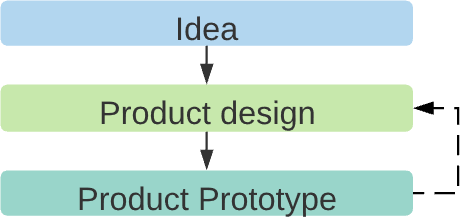
\includegraphics[width=8cm]{36}
\caption{\Large Sectioned diagram regarding product development  產品開發剖面圖}\label{fig.36}
\end{center}
\end{figure}
\fontsize{12}{2.5pt}\selectfont {It is at this point that the utilization of the Odoo software can officially take place. The
first step is to understand what the subject of production is as far as product items are
concerned. There are two takes in how to do this:
▪ The first is to consider the prototype an early revision of the final product, that is
the prototype item created in Odoo would be the same as the final product item
with revisions been carried out during development. That would be the
recommended if the prototype is achieved by identical means to the ones used in
the final production. An example of this approach would be if the product is
simple enough that product and production aspects of development can be carried
out together.
▪ The second one is to consider the prototype as a separate item from the final
product - this is the path was taken in this simulation. The main reason for this
decision was that the ways in which our prototype production were carried out
differed from the final production since 3D printing was used for the prototypes.
Starting from the root, a product item called PROTO Alpha Case (Figure 37) was created
(Alpha Case being the name of the product). From this point on we will refer to prototype
products as ‘proto item’. As we can see, this allows for a nice representation of the proto
item. Since it is a prototype, it will not be marked as something that can be sold or purchased,
and sales price will be set to 0 since it is unimportant. This proto item will be used to connect
the different aspects of its development but for now it is left alone.}\\[1pt]

\fontsize{12}{2.5pt}\selectfont {此時即可正式使用 Odoo 軟體。這第一步是了解生產的主題是什麼,就產品項目而言擔心的。如何做到這一點有兩種做法:▪ 首先是將原型視為最終產品的早期修訂版,即在 Odoo 中創建的原型項目將與最終產品項目相同在開發過程中進行了修改。那將是如果原型是透過與中使用的相同的方式實現的,則推薦最終的製作。這種方法的一個例子是,如果產品是夠簡單,可以進行產品和生產的開發一起出去。▪ 第二個是將原型視為獨立於最終產品的單獨項目產品 - 這是本次模擬中所採取的路徑。造成這種情況的主要原因決定是我們的原型生產的方式由於原型使用了 3D 列印,因此與最終產品有所不同。從根開始,創建了一個名為 PROTO Alpha Case(圖 37)的產品項(Alpha Case 是產品的名稱)。從現在開始我們將參考原型產品作為「原型項目」。正如我們所看到的,這可以很好地表示原型物品。由於它是原型,因不會標記為可以出售或購買的東西,銷售價格將設定為 0,因為它不重要。此原型項目將用於連接其發展的不同方面,但目前它被擱置了。}\\[1pt]
\begin{figure}[hbt!]
\begin{center}
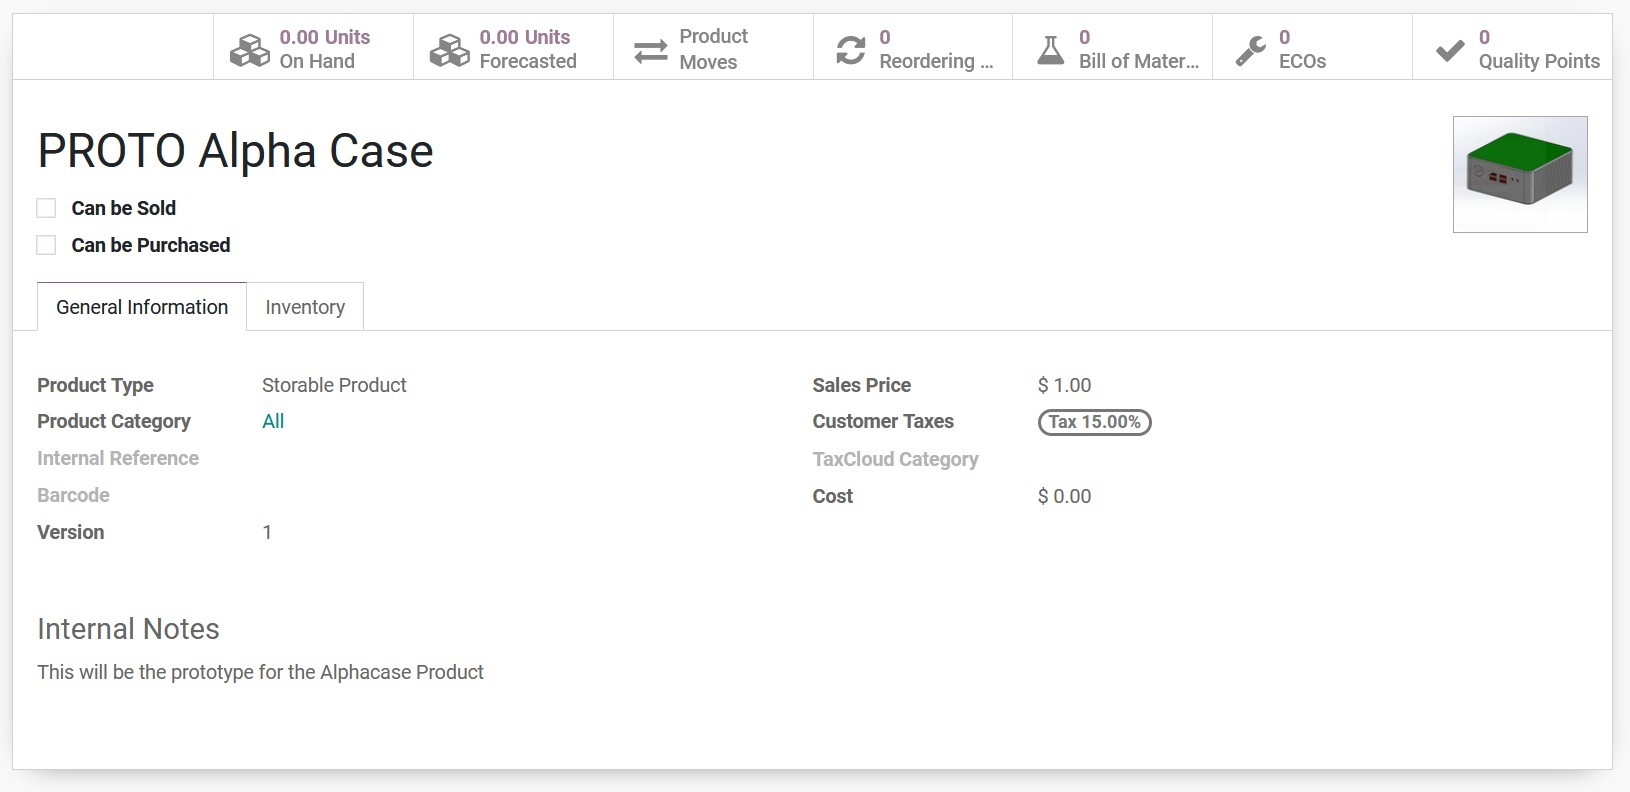
\includegraphics[width=10cm]{37}
\caption{\Large Image of the prototype product item  原型產品項目的圖像圖}\label{fig.37}
\end{center}
\end{figure}
\fontsize{12}{2.5pt}\selectfont {As we have previously stablished in chapter 3, the product will consist of 3 pieces Part A, Part B and Part C. These need to be prototyped and created as products as well so that they can be added to the bill of materials of the PROTO Alpha Case. Finally, it was decided to use specific plastic filaments (see section 4.1.1) for the 3D printing of PROTO Part A and PROTO Part B and C and these need to be added as products as well (Figure 38).}\\[1pt]

\fontsize{12}{2.5pt}\selectfont {正如我們之前在第 3 章中所確定的,該產品將由 3 部分組成:A 部分、B 部分和 C 部分。這些也需要進行原型設計並創建為產品,以便可以將它們添加到 PROTO 的物料清單中阿爾法案例。最後,決定使用特定的塑膠絲(請參閱第 4.1.1 節)來 3D 列印原型 A 部分以及原型 B 和 C 部分,並且這些也需要作為產品添加(圖 38)。}\\[1pt]
\begin{figure}[hbt!]
\begin{center}
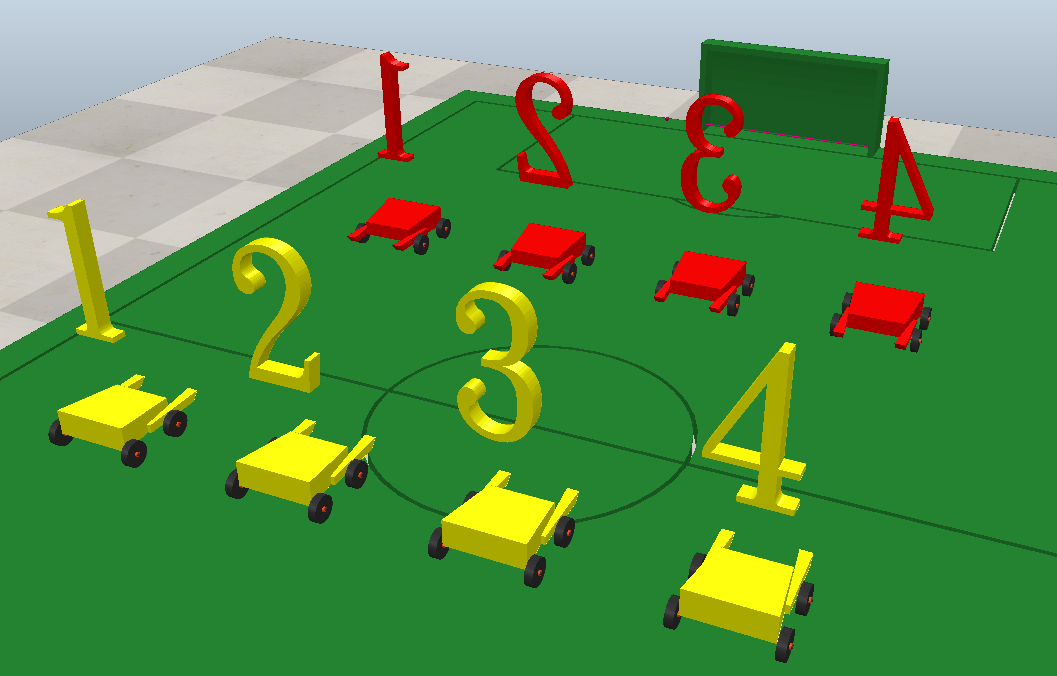
\includegraphics[width=10cm]{38}
\caption{\Large Overview of Product class items for prototype 原型產品類別項目概述}\label{fig.38}
\end{center}
\end{figure}
\fontsize{12}{2.5pt}\selectfont {At this point, the relevant product items for the prototyping of the Alpha Case were finished, which makes possible the creation of the its relevant BOMs. There are 3 of them and they follow the structure in (Figure 39)}\\[1pt]

\fontsize{12}{2.5pt}\selectfont {至此,Alpha Case原型製作的相關產品項目已經完成,可以創造其相關的BOM。其中有 3 個,它們遵循(圖 39)中的結構}\\[1pt]
\newpage
\begin{figure}[hbt!]
\begin{center}
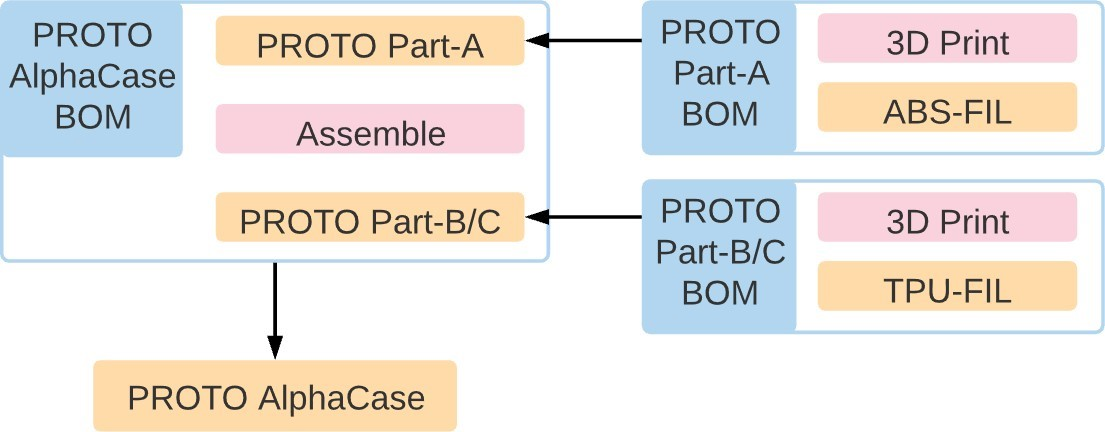
\includegraphics[width=10cm]{39}
\caption{\Large BOM diagrams for prototyping  用於原型設計的 BOM 圖}\label{fig.39}
\end{center}
\end{figure}

\fontsize{12}{2.5pt}\selectfont {Something worth mentioning is that Odoo used the kit option (Figure 40) on the item to infer that this product is a component of another product. This is very interesting because it automatically creates dependencies between the product items for production}\\[1pt]

\fontsize{12}{2.5pt}\selectfont {值得一提的是,Odoo 在該商品上使用了套件選項(圖 40)來推斷該產品是另一個產品的組件。這非常有趣,因為它會自動在生產的產品項目之間建立依賴關係。}\\[1pt]
\begin{figure}[hbt!]
\begin{center}
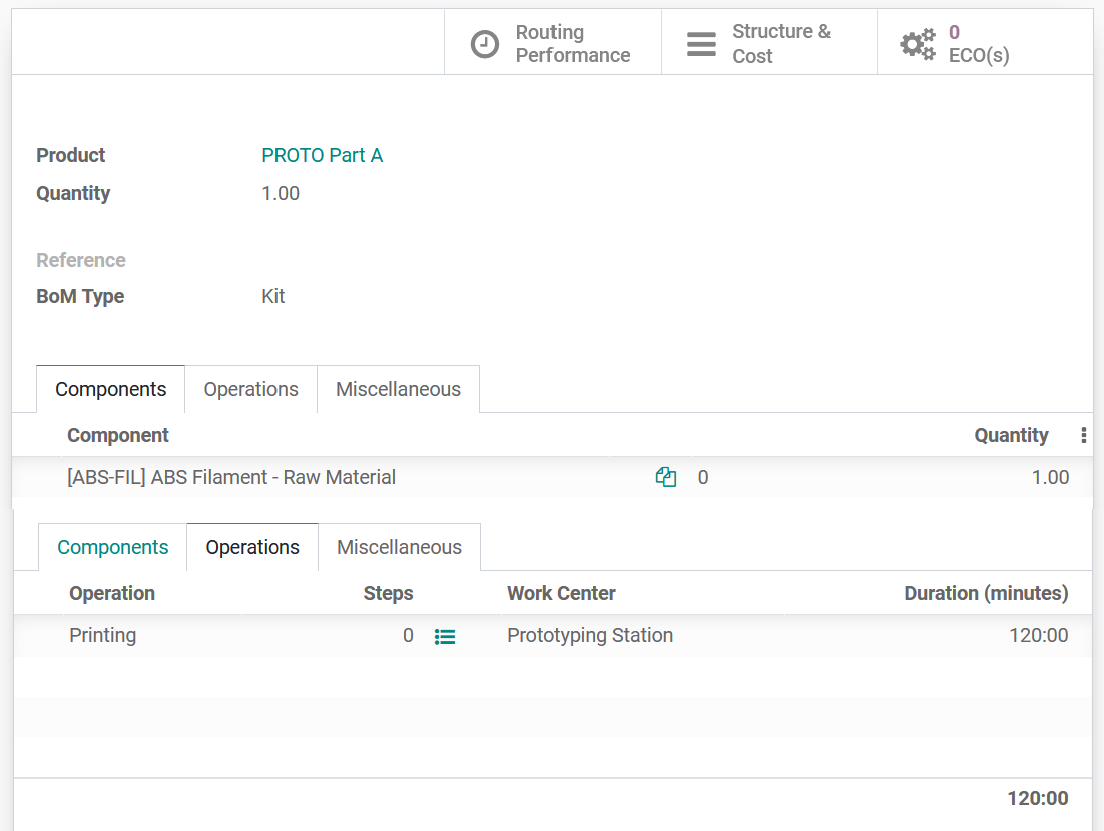
\includegraphics[width=15cm]{40}
\caption{\Large Image of the prototype product BOM (Part-A)  原型產品 BOM(A 部分)}\label{fig.40}
\end{center}
\end{figure}
\fontsize{12}{2.5pt}\selectfont {As the reader can see (Figure 41), while making the BOMs it is simple to create the specific operation items necessary for the manufacturing procedure and specify its work center. One of the best functionalities regarding MES in Odoo is the ability to track the time of operations based on default duration. This can be dynamically changed based on tracked time or set manually. It is also in the operation item that we can add instruction files for the operation. Even though it is limited to PDF text or a link to a google slides file, this is one of the few opportunities presented by Odoo for file management connected directly to an item.}\\[1pt]


\fontsize{12}{2.5pt}\selectfont {如讀者所見(圖 41),在製作 BOM 時,可以輕鬆創建製造過程所需的特定操作項目並指定其工作中心。 Odoo 中 MES 的最佳功能之一是能夠根據預設持續時間追蹤操作時間。這可以根據追蹤時間動態更改或手動設定。也是在操作項中我們可以新增操作的指令檔。儘管它僅限於 PDF 文字或 Google 幻燈片文件的鏈接,但這也是 Odoo 為直接連接到專案的文件管理提供的少數機會之一。}\\[1pt]
\begin{figure}[hbt!]
\begin{center}
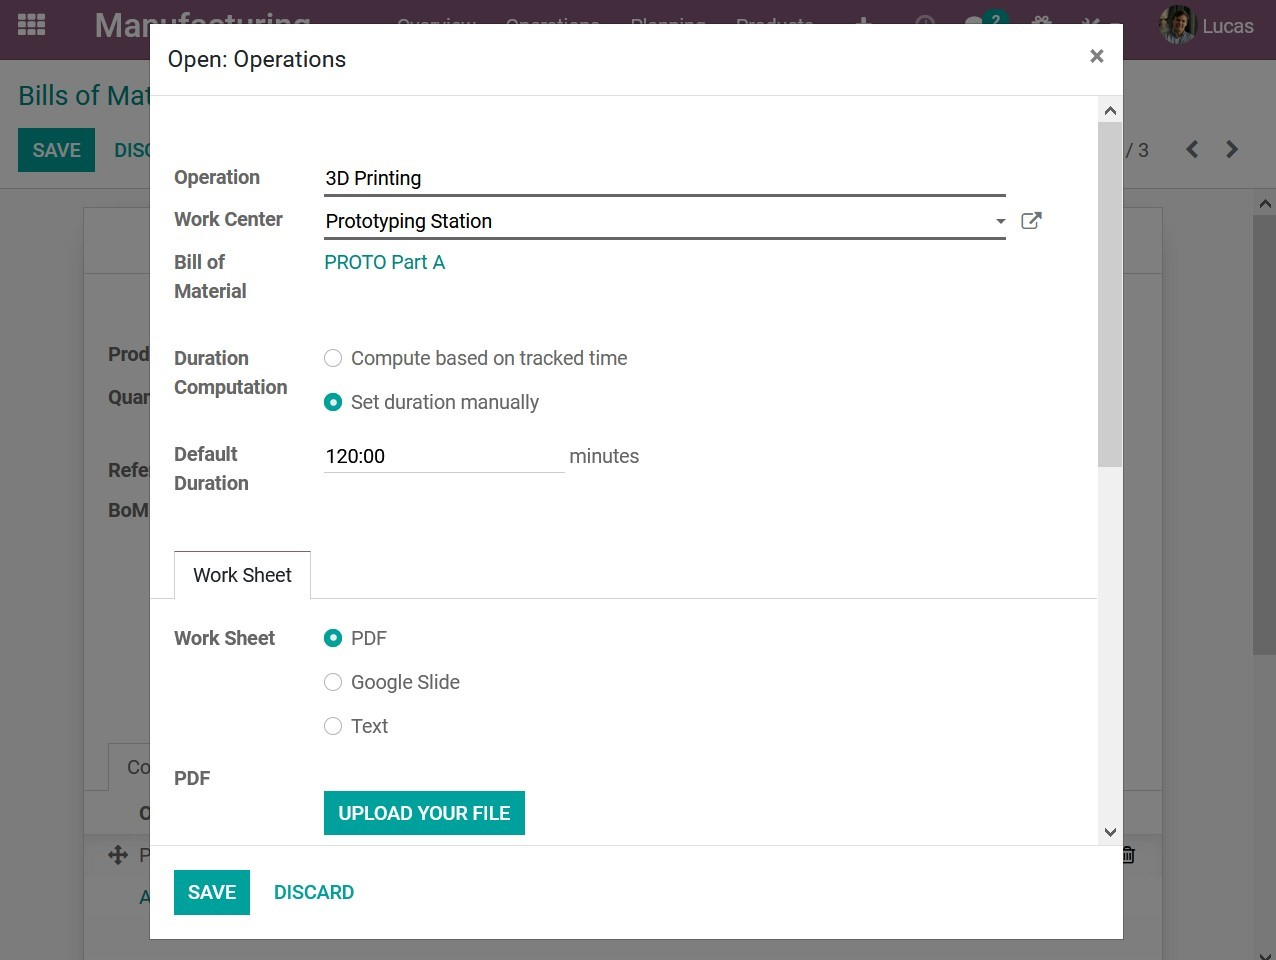
\includegraphics[width=10cm]{41}
\caption{\Large Image of the prototype product BOM (Part-A)  原型產品 BOM(A 部分)}\label{fig.41}
\end{center}
\end{figure}

\begin{figure}[hbt!]
\begin{center}
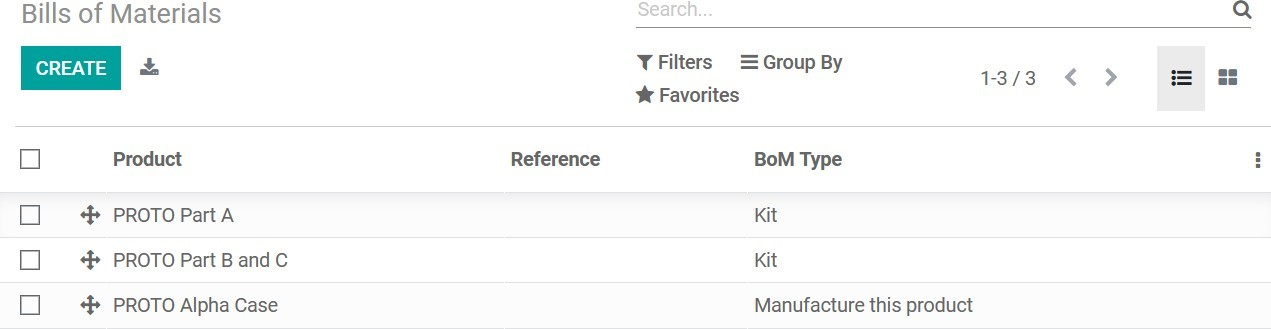
\includegraphics[width=10cm]{42}
\caption{\Large Overview of BOMs created for prototyping  為原型設計創建的 BOM 概述}\label{fig.42}
\end{center}
\end{figure}
\fontsize{12}{2.5pt}\selectfont {Speaking of this lack of upload opportunities, we can notice that while making the product item there was no way to directly upload files regarding the product to the item. In our case, we have the CAD files regarding the parts that we are prototyping, to not be able to upload these files in any way would be a complete failure from a PLM perspective. Thankfully there is a workaround. As explained in section 5.1.3.5, the ECO is an item that is linked to either product items or BOMs and allow uploaded files to be attached to it. It is a minor workaround but basically means that if we want to upload our CAD files to the items in any significative manner, we need to emit an ECO even if there is no “change” being made.}\\[1pt]

\fontsize{12}{2.5pt}\selectfont {說到缺乏上傳機會,我們可以注意到,在製作產品項目時,無法直接將有關產品的文件上傳到該項目。在我們的例子中,我們擁有與我們正在製作原型的零件相關的 CAD 文件,從 PLM 的角度來看,如果無法以任何方式上傳這些文件,那將是徹底的失敗。值得慶幸的是,有一個解決方法。如第 5.1.3.5 節所述,ECO 是連結到產品項目或 BOM 的項目,並允許將上傳的檔案附加到其上。這是一個較小的解決方法,但基本上意味著,如果我們想以任何有意義的方式將 CAD 檔案上傳到項目,即使沒有進行“更改”,我們也需要發出 ECO。}\\[1pt]
\newpage
\begin{figure}[hbt!]
\begin{center}
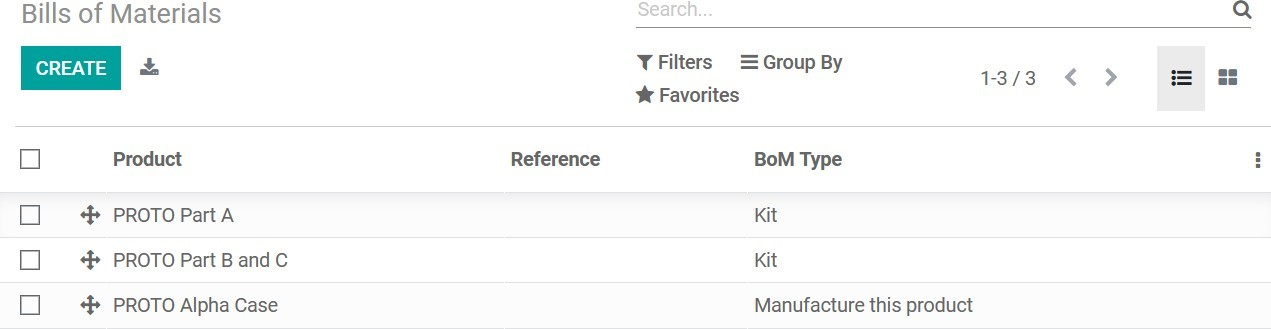
\includegraphics[width=10cm]{42}
\caption{\Large Overview of BOMs created for prototyping  為原型設計創建的 BOM 概述}\label{fig.42}
\end{center}
\end{figure}
\fontsize{12}{2.5pt}\selectfont {Speaking of this lack of upload opportunities, we can notice that while making the product item there was no way to directly upload files regarding the product to the item. In our case, we have the CAD files regarding the parts that we are prototyping, to not be able to upload these files in any way would be a complete failure from a PLM perspective. Thankfully there is a workaround. As explained in section 5.1.3.5, the ECO is an item that is linked to either product items or BOMs and allow uploaded files to be attached to it. It is a minor workaround but basically means that if we want to upload our CAD files to the items in any significative manner, we need to emit an ECO even if there is no “change” being made.}\\[1pt]

\fontsize{12}{2.5pt}\selectfont {說到缺乏上傳機會,我們可以注意到,在製作產品項目時,無法直接將有關產品的文件上傳到該項目。在我們的例子中,我們擁有與我們正在製作原型的零件相關的 CAD 文件,從 PLM 的角度來看,如果無法以任何方式上傳這些文件,那將是徹底的失敗。值得慶幸的是,有一個解決方法。如第 5.1.3.5 節所述,ECO 是連結到產品項目或 BOM 的項目,並允許將上傳的檔案附加到其上。這是一個較小的解決方法,但基本上意味著,如果我們想以任何有意義的方式將 CAD 檔案上傳到項目,即使沒有進行“更改”,我們也需要發出 ECO。}\\[1pt]
\newpage
\begin{figure}[hbt!]
\begin{center}
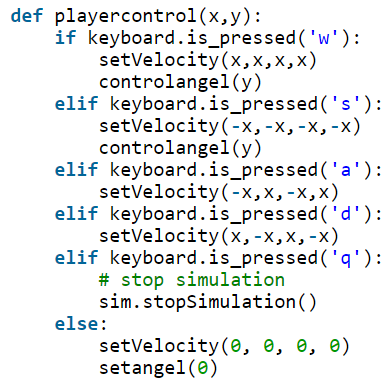
\includegraphics[width=10cm]{43}
\caption{\Large ECO example  生態範例}\label{fig.43}
\end{center}
\end{figure}

\fontsize{12}{2.5pt}\selectfont {It can only be assumed that this was part of Odoo’s team strategy to implement PLM as an external application in its ERP base. It is reasonable, but still, this is one of the few aspects of this software interface that is not as straightforward. It is an extremely valuable feature, but it is somewhat hidden. The documents icon appears in the top right corner (Figure 43) only after the ECO is created and saved.}\\[1pt]


\fontsize{12}{2.5pt}\selectfont {只能假設這是 Odoo 團隊策略的一部分,即將 PLM 作為其 ERP 基礎中的外部應用程式實施。這是合理的,但這仍然是該軟體介面中少數幾個不那麼簡單的方面之一。這是一個非常有價值的功能,但它有些隱藏。僅在建立並儲存 ECO 後,文件圖示才會出現在右上角(圖 43)。}\\[1pt]
\newpage
\begin{figure}[hbt!]
\begin{center}
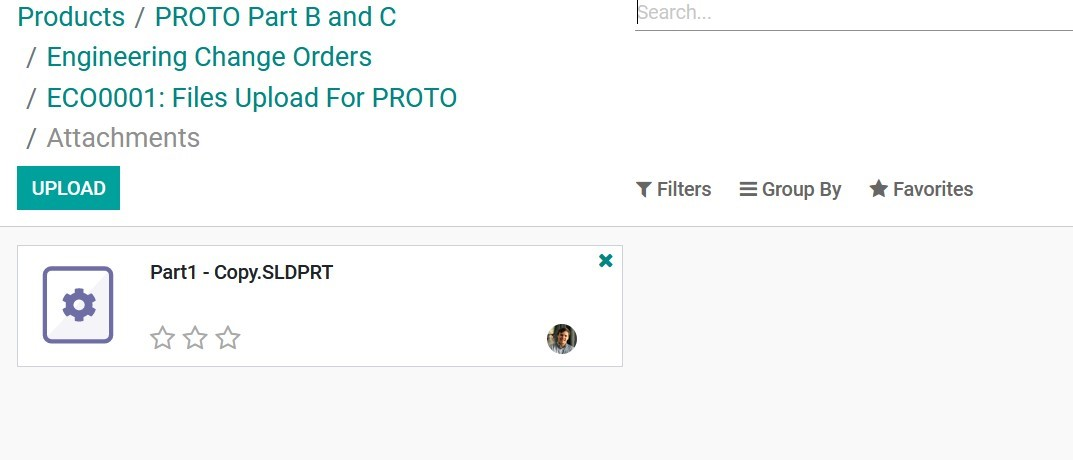
\includegraphics[width=10cm]{44}
\caption{\Large Overview of attached files to ECO ECO 附文件概述}\label{fig.44}
\end{center}
\end{figure}
\fontsize{12}{2.5pt}\selectfont {Since there is no direct integration between Odoo and the CAD software, uploading the file do not cause any automatic change to the product metadata. This is not ideal from the PLM perspective, still, it is a well implemented feature. By allowing product items to link directly to not only one existing ECO but to the list of all ECOs ever applied to the item, the software does well in tracking version control and development.

Something interesting that can be done for the sake of process control is adding quality control points to operations. This allows the responsible personnel to give feedback during the production regarding concerning points to the engineering team. In our case, we are concerned about 3D printing warping. This is something that happens when temperature varies to much during the 3D printing procedure. To this end a Quality Control Point item will be created (Figure 45) that will enquire with the operator to check if there is warping in the piece and mark pass or fail.
}\\[1pt]

\fontsize{12}{2.5pt}\selectfont {由於 Odoo 和 CAD 軟體之間沒有直接集成,因此上傳檔案不會導致產品元資料發生任何自動變更。從 PLM 的角度來看,這並不理想,但它仍然是實施良好的功能。透過允許產品項目不僅直接連結到一個現有的 ECO,而且連結到曾經應用於該項目的所有 ECO 的列表,該軟體在追蹤版本控制和開發方面表現良好。

為了過程控制可以做的一些有趣的事情是在操作中添加品質控制點。這使得負責人員可以在生產過程中向工程團隊提供有關要點的回饋。在我們的案例中,我們擔心 3D 列印翹曲。這是 3D 列印過程中溫度變化過大時會發生的情況。為此,將建立一個品質控制點專案(圖 45),該專案將詢問操作員以檢查工件是否存在翹曲並標記為通過或失敗。}\\[1pt]
\newpage
\begin{figure}[hbt!]
\begin{center}
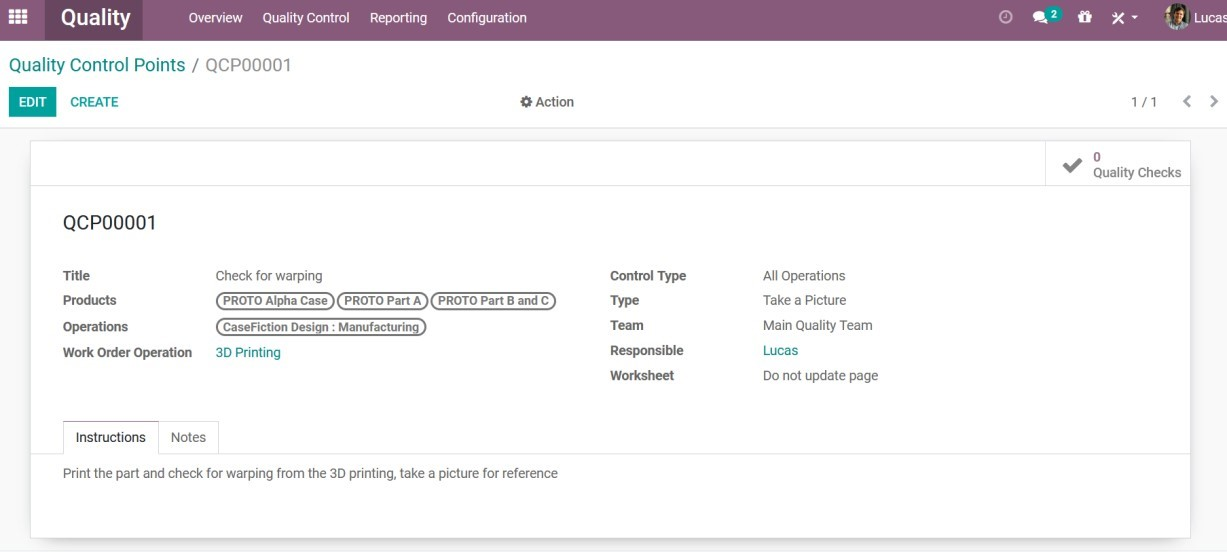
\includegraphics[width=10cm]{45}
\caption{\Large Quality Control Point item for the prototype production 原型生產的品質控制點項目}\label{fig.45}
\end{center}
\end{figure}
\fontsize{12}{2.5pt}\selectfont {The last step of a prototype cycle would be the production of prototypes for testing and evaluation. Production is something quite straightforward in Odoo and really the point where everything we have done before come together. The metadata and the items that have been created allow us to start the Manufacturing Order (MO) (Figure 46). This, in turn, pull the necessary workorders from the operations and components listed in the BOM. The workorders appear for manufacturing operators and production can commence/be tracked.
}\\[1pt]

\fontsize{12}{2.5pt}\selectfont {原型週期的最後一步是生產用於測試和評估的原型。在 Odoo 中,製作是相當簡單的事情,也是我們之前所做的一切都匯集在一起的地方。已建立的元資料和項目使我們能夠啟動製造訂單 (MO)(圖 46)。這反過來又從 BOM 中列出的操作和組件中提取必要的工作訂單。工作訂單會出現給製造操作員,並且可以開始/追蹤生產。}\\[1pt]
\newpage
\begin{figure}[hbt!]
\begin{center}
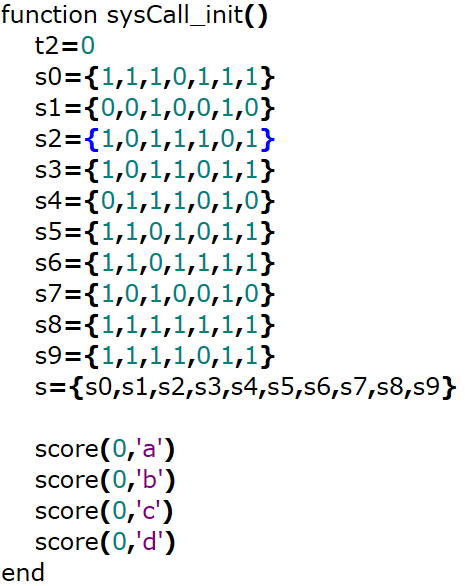
\includegraphics[width=10cm]{46}
\caption{\Large Depiction of the manufacturing order 製造訂單的描述}\label{fig.46}
\end{center}
\end{figure}
\fontsize{12}{2.5pt}\selectfont {For the most part this operation is very well automated and clear. There are however a few problems that are result of structural changes from Odoo V13 to Odoo V14. For a long time, the software ordered the operations to be carried out using an extra item class called ‘Route’. These were a fundamental part of how the product moved within the inventory and manufacturing, but for some reason, was dropped in the manufacturing aspect of the new version in favor of a simplified sequence data built into the BOM. As of the writing of this work, there have been reports of problems and confusions regarding how that works, which are aggravated by the fact that material explaining the use of this functionality are either nonexistent or still referencing old versions of the software (in which ‘routes’ are still in use).

The avid reader will notice in Figure 47 that the order in which operations are being made available are not in the correct sequence. This is due to exactly this problem and for now the
 
only solution is to count on the awareness of the operators regarding the order of production or manually scheduling the operations in the plan tab. During the period of research for this work (before Odoo V14) familiarization experiments were made in which there were no problem of this nature. In addition, there are examples online even from Odoo website demonstrating the use of routes and how they are useful for this exact situation.
}\\[1pt]

\fontsize{12}{2.5pt}\selectfont {在大多數情況下,此操作非常自動化且清晰。然而,從 Odoo V13 到 Odoo V14 的結構變化導致了一些問題。長期以來,軟體命令使用名為「Route」的額外項目類別來執行操作。這些是產品在庫存和製造中移動的基本部分,但由於某種原因,在新版本的製造方面被放棄,轉而採用 BOM 中內建的簡化序列資料。在撰寫本文時,已經有關於其工作原理的問題和混亂的報告,而解釋此功能的使用的材料要么不存在,要么仍然引用舊版本的軟體(其中“路線仍在使用中)。

熱心的讀者會注意到圖 47 中操作的可用順序不正確。這正是由於這個問題造成的,目前
 
唯一的解決方案是依靠操作員對生產訂單的了解或在計劃選項卡中手動安排操作。在這項工作的研究期間(Odoo V14 之前)進行了熟悉實驗,其中不存在這種性質的問題。此外,Odoo 網站上也有線上範例,演示了路線的使用以及它們如何在這種具體情況下發揮作用。}\\[1pt]
\newpage
\begin{figure}[hbt!]
\begin{center}
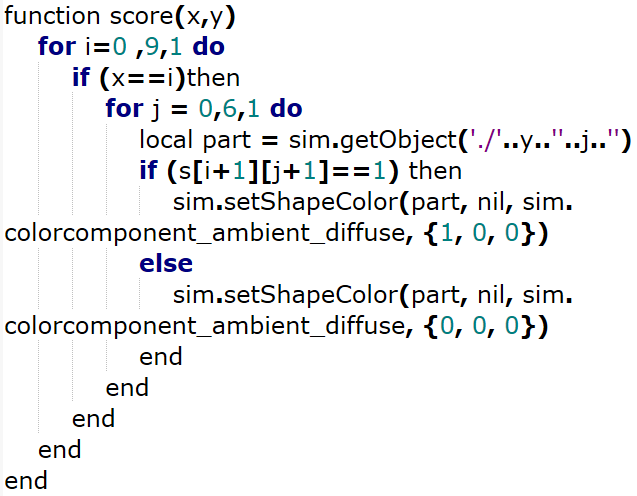
\includegraphics[width=10cm]{47}
\caption{\Large Overview of the resulted Work Orders 結果工單概述}\label{fig.47}
\end{center}
\end{figure}
\fontsize{12}{2.5pt}\selectfont {The problem has been reported by other people (Figure 48) to the Odoo company and is been and hopefully it will be resolved shortly (this is after all a extremelly recent version of the software). That been said, it is a problem even if it is a minor one.
}\\[1pt]

\fontsize{12}{2.5pt}\selectfont {其他人已向 Odoo 公司報告了該問題(圖 48),並希望很快就能得到解決(畢竟這是該軟體的最新版本)。話雖如此,即使這是一個小問題,也是一個問題。}\\[1pt]
\begin{figure}[hbt!]
\begin{center}
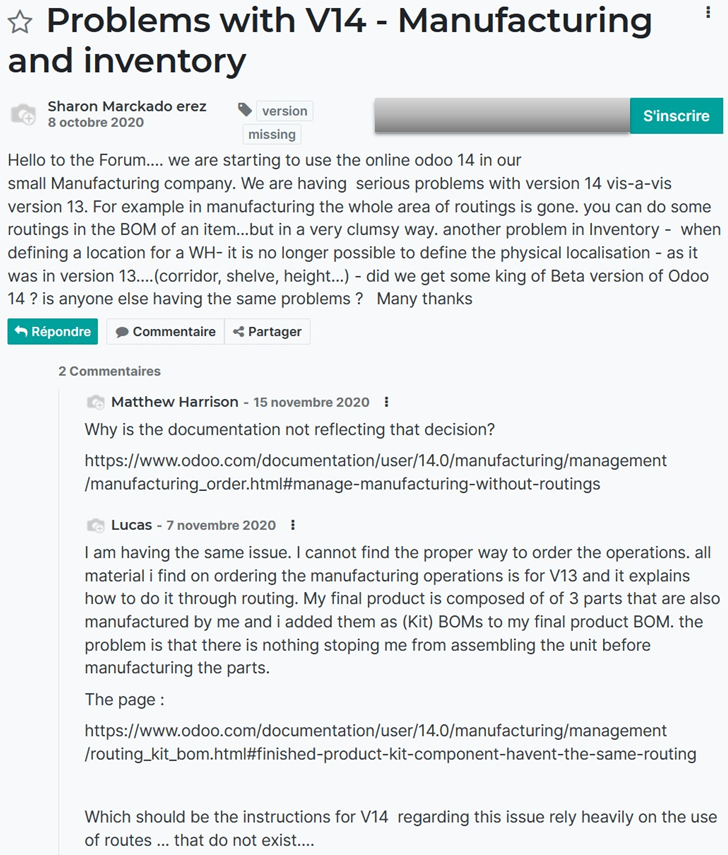
\includegraphics[width=10cm]{48}
\caption{\Large mage of Odoo forum question regarding routes  Odoo 論壇法師關於路線的問題}\label{fig.48}
\end{center}
\end{figure}
\fontsize{12}{2.5pt}\selectfont {The manufacturing process was repeated 7 times (Figure 49) to simulate a small batch of prototypes for testing and tolerance checking. It is rare to get a perfect prototype in the first batch, for this reason it was chosen to represent correction through the simulation. In this simulation this problem was a fit problem that resulted in a change of dimension of PROTO Part A.
}\\[1pt]

\fontsize{12}{2.5pt}\selectfont {製造過程重複 7 次(圖 49),以模擬小批量原型進行測試和公差檢查。在第一批中獲得完美原型的情況很少見,因此選擇它來代表透過模擬進行修正。在此模擬中,該問題是一個擬合問題,導致原型 A 部分的尺寸發生變化。}\\[1pt]
\begin{figure}[hbt!]
\begin{center}
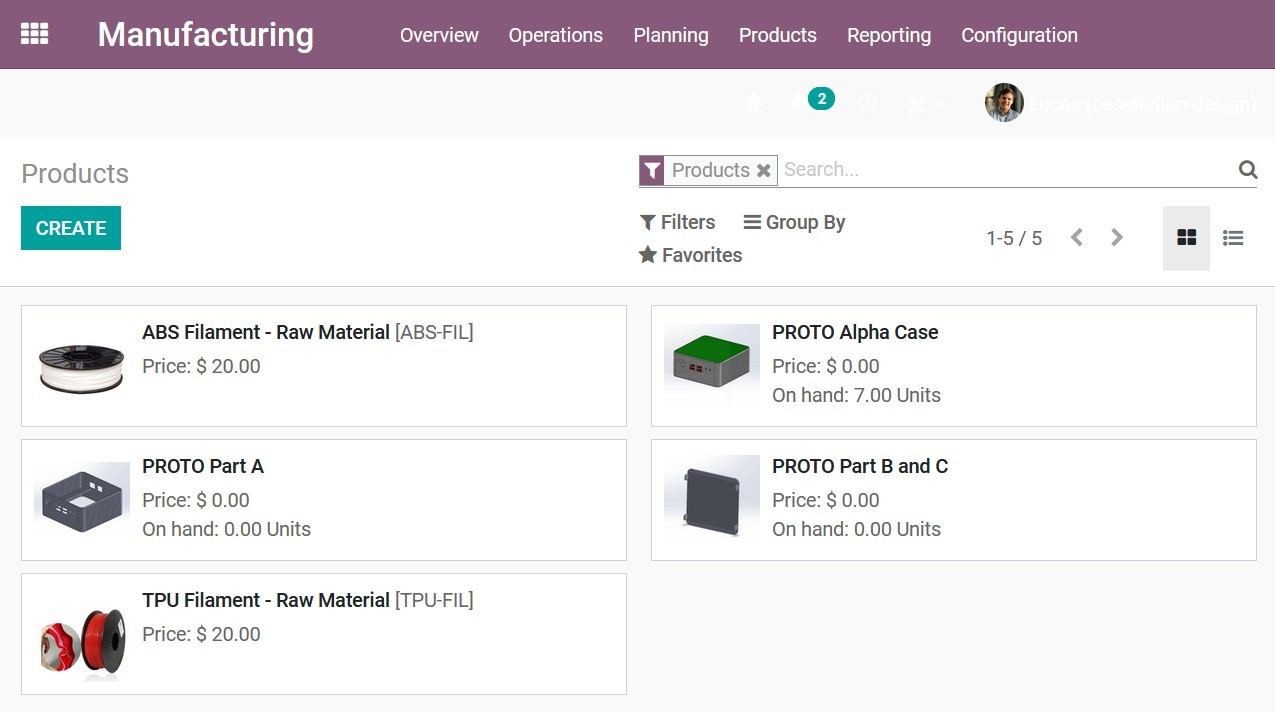
\includegraphics[width=10cm]{49}
\caption{\Large Overview of the products after manufacturing 結果工單概述}\label{fig.49}
\end{center}
\end{figure}
\newpage
\fontsize{12}{2.5pt}\selectfont {This give us the opportunity to use ECOs for their actual purpose, stablish and control a change to the product item. The changes to be carried out were on the CAD file regarding the product item. As before we can start the ECO and fill in the description, then the files are uploaded, and the ECO (Figure 50) goes through necessary validation before been made effective.
}\\[1pt]

\fontsize{12}{2.5pt}\selectfont {這使我們有機會將 ECO 用於其實際目的、建立和控制產品項目的變更。要進行的變更是在有關產品項目的 CAD 檔案上進行的。與之前一樣,我們可以啟動 ECO 並填寫描述,然後上傳文件,ECO(圖 50)經過必要的驗證後才會生效。}\\[1pt]
\newpage
\begin{figure}[hbt!]
\begin{center}
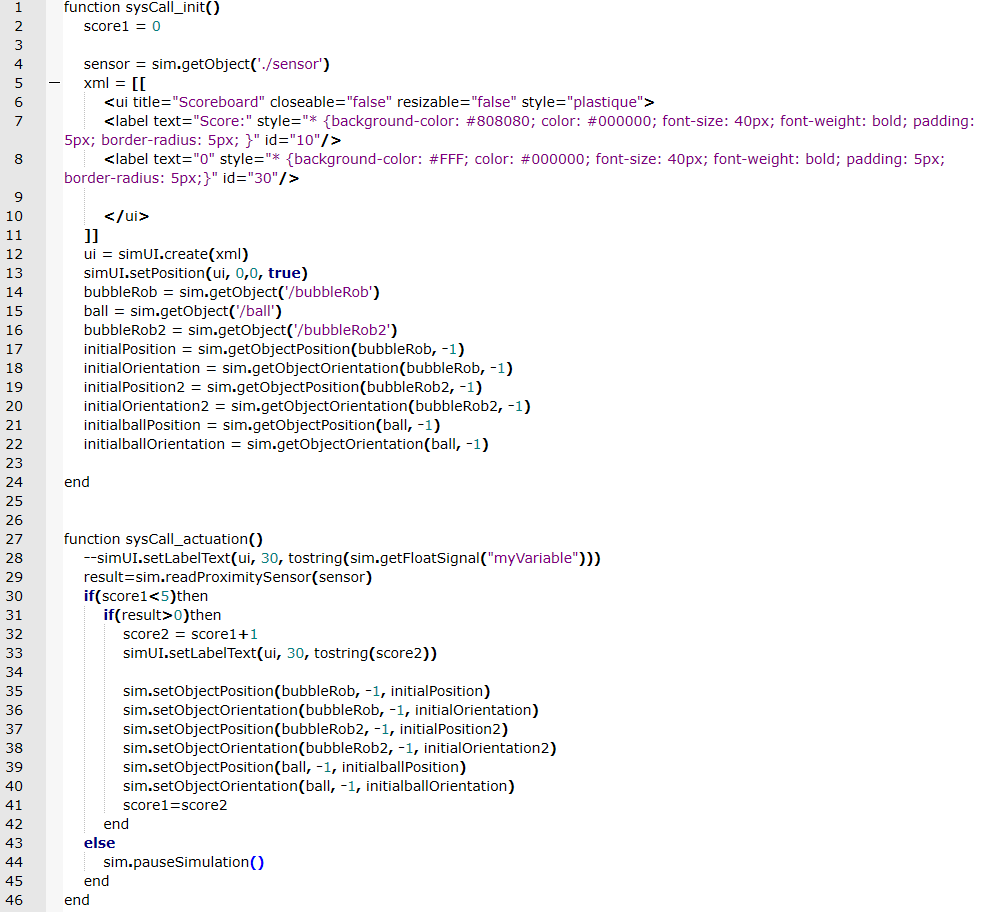
\includegraphics[width=10cm]{50}
\caption{\Large Depiction of the validation of the ECO ECO 驗證描述}\label{fig.50}
\end{center}
\end{figure}
\fontsize{12}{2.5pt}\selectfont {The validation procedure basically is set to ask for validation of someone with proper access permissions or specific personnel. In this case, the master account was used to validate and make effective as can be seen from the log in the right side of the image. Once the change
 
is applied you can see that the product item version has been iterated to version 2 as well as a new ECO has been added to the list of ECOs linked to the item (Figure 51).
}\\[1pt]

\fontsize{12}{2.5pt}\selectfont {驗證程序基本上設定為要求具有適當存取權限的人員或特定人員進行驗證。在本例中,主帳戶用於驗證並生效,從圖像右側的日誌可以看出。一旦改變套用後,您可以看到產品項目版本已迭代到版本 2,並且新的 ECO 已新增至連結到該項目的 ECO 清單(圖 51)。}\\[1pt]
\begin{figure}[hbt!]
\begin{center}
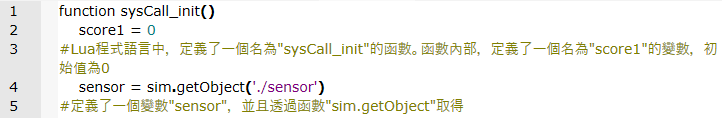
\includegraphics[width=10cm]{51}
\caption{\Large Depiction of changes provoked by the ECO to product item  描述 ECO 對產品項目所引起的變化}\label{fig.51}
\end{center}
\end{figure}
\fontsize{12}{2.5pt}\selectfont {That update is followed by another batch of prototypes, the cycle would continue until the prototypes produced satisfy the criteria stablished by the design team. In the case of this simulation it was assumed that one correction was representative enough of this process. This finalizes the development from idea to prototype.
}\\[1pt]

\fontsize{12}{2.5pt}\selectfont {更新之後是另一批原型,循環將繼續,直到生產的原型滿足設計團隊制定的標準。在此模擬的情況下,假設一次校正足以代表該過程。這就完成了從想法到原型的開發。}\\[1pt]









